%%%%%%%%%%%%%%%%%%%%%%%%%%%%%%%%%%%%%%%%%%%%%%%%%%%%%%%%%%%%%%%%%%%%%%%%
% Mostly grammarly'd
\chapter{Fundamentals}
\label[section]{sec:fundamentals}

\begin{figure}[ht]
    \begin{subfigure}{.49\textwidth}
        \centering
        \includegraphics[scale=.125]{figures/Fundamentals/WavesVector.png}
        \caption{}
    \end{subfigure}
    \begin{subfigure}{.49\textwidth}
        \centering
        \includegraphics[scale=.125]{figures/Fundamentals/SpiralSinkVector.png}
        \caption{}
    \end{subfigure}
    \caption{
        Two vector fields visualized using a vector plot.
        The field in (a) is defined by $u(x,y) = (1, \sin(x))^T$,
        the field used for (b) is $u(x,y) = (-0.5x -y, 0.5x - y)^T$.
        %  [-self._xshear, -1, 0], [self._xshear, -1, 0]
    }
    \label[figure]{fig:fundamentals_1}
\end{figure}

In this section, we describe the elementary components used in the remainder of this thesis.
Since this work is about the placement of streamlines in vector fields,
we start with the fundamentals of \textit{vector field visualization} in \Cref{sec:VFV}.
Our algorithm uses an image-guided base, so we also need topics from the area of \textit{image processing} in \Cref{sec:IP}.
We conclude this chapter with a brief overview of the \textit{roots of unity} in \Cref{sec:ROU}
because we use them to develop a prototype in \Cref{sec:3D}.


\section{Vector Field Visualization}
\label[section]{sec:VFV}
This field revolves around how to make spatial scalar data more accessible to human understanding.
We focus on the visualization of two-dimensional fields, two examples can be seen in \Cref{fig:fundamentals_1}.
\newpage

\subsection{Vector Fields}
A vector field represents how vectorized elements act over a spatial domain.
Concerning vector fields representing flow, for every point in a domain
we can obtain the flow velocity at that point.

More formally, we can define a vector field as a map from $n$-dimensional scalars to $m$-dimensional scalars.
We can write it as an $n$-$m$-valued function, and in this thesis,
we will only care about cases of $n=m$ in two and three dimensions.
There are several ways to obtain such fields, one is via an algebraic definition
such as $u(x,y) = (1, \sin(x))^T$, giving us a field like the one seen in \Cref{fig:fundamentals_1}.
If we want our velocity to not only depend on spatial input
but also on another scalar like a time component $t$, we write this as $u(x,y,t)$ for the 2D case.       
We call vector fields \textit{steady} if they are not time-dependent;
otherwise, we refer to them as \textit{unsteady}.
Another distinction is \textit{continuity}, which is analogous to the algebraic definition of other functions.
The fields in this work are all going to be continuous.

\newpage

\subsection{Critical Points}
\begin{figure}[t]
    \centering
    \begin{subfigure}{.49\textwidth}
        \centering
        \includegraphics[scale=.125]{figures/Fundamentals/SinkVector.png}
        \caption{}
    \end{subfigure}
    \centering
    \begin{subfigure}{.49\textwidth}
        \centering
        \includegraphics[scale=.125]{figures/Fundamentals/SaddleVector.png}
        \caption{}
    \end{subfigure}
    \caption{
        (a) Vector plot of a sink defined by $u(x,y) = (-x, -y)^T$.
        (b) Vector plot of a saddle defined by $u(x,y) = (x-y,-x-y)^T$.
    }
    \label[figure]{fig:fundamentals_sink}
\end{figure}

A vector field can have points with distinct characteristics, called critical points.
In the 2D case, only four commonly used critical points exist, which we briefly describe here.
\paragraph{Source}
Given a field such as $u(x,y) = (x,y)$, at every point applies a force away from the origin.
If we think about this as a non-compressible flow,
this is equivalent to matter being created at the point $(0,0)$ and flowing outward.
Hence, we refer to such points as \textit{sources}.
\paragraph{Sink}
Similarly, $u(x,y) = (-x,-y)$ would give us a \textit{sink} at $(0,0)$,
equivalent to destroying liquid flowing inward.
This is shown in \Cref{fig:fundamentals_sink}.
\paragraph{Saddle}
A saddle is an area where matter is pinched in one direction and stretched in another, e.g. in a field defined by $u(x,y) = (-x,y)$.
\paragraph{Periodic Orbit}
$u(x,y) = (-y,x)$ creates circular paths around the origin where, after traveling a certain distance, a particle arrives at the point it started at.
These critical points are called \textit{periodic orbits}.

\newpage
\begin{figure}[t]
    \centering
    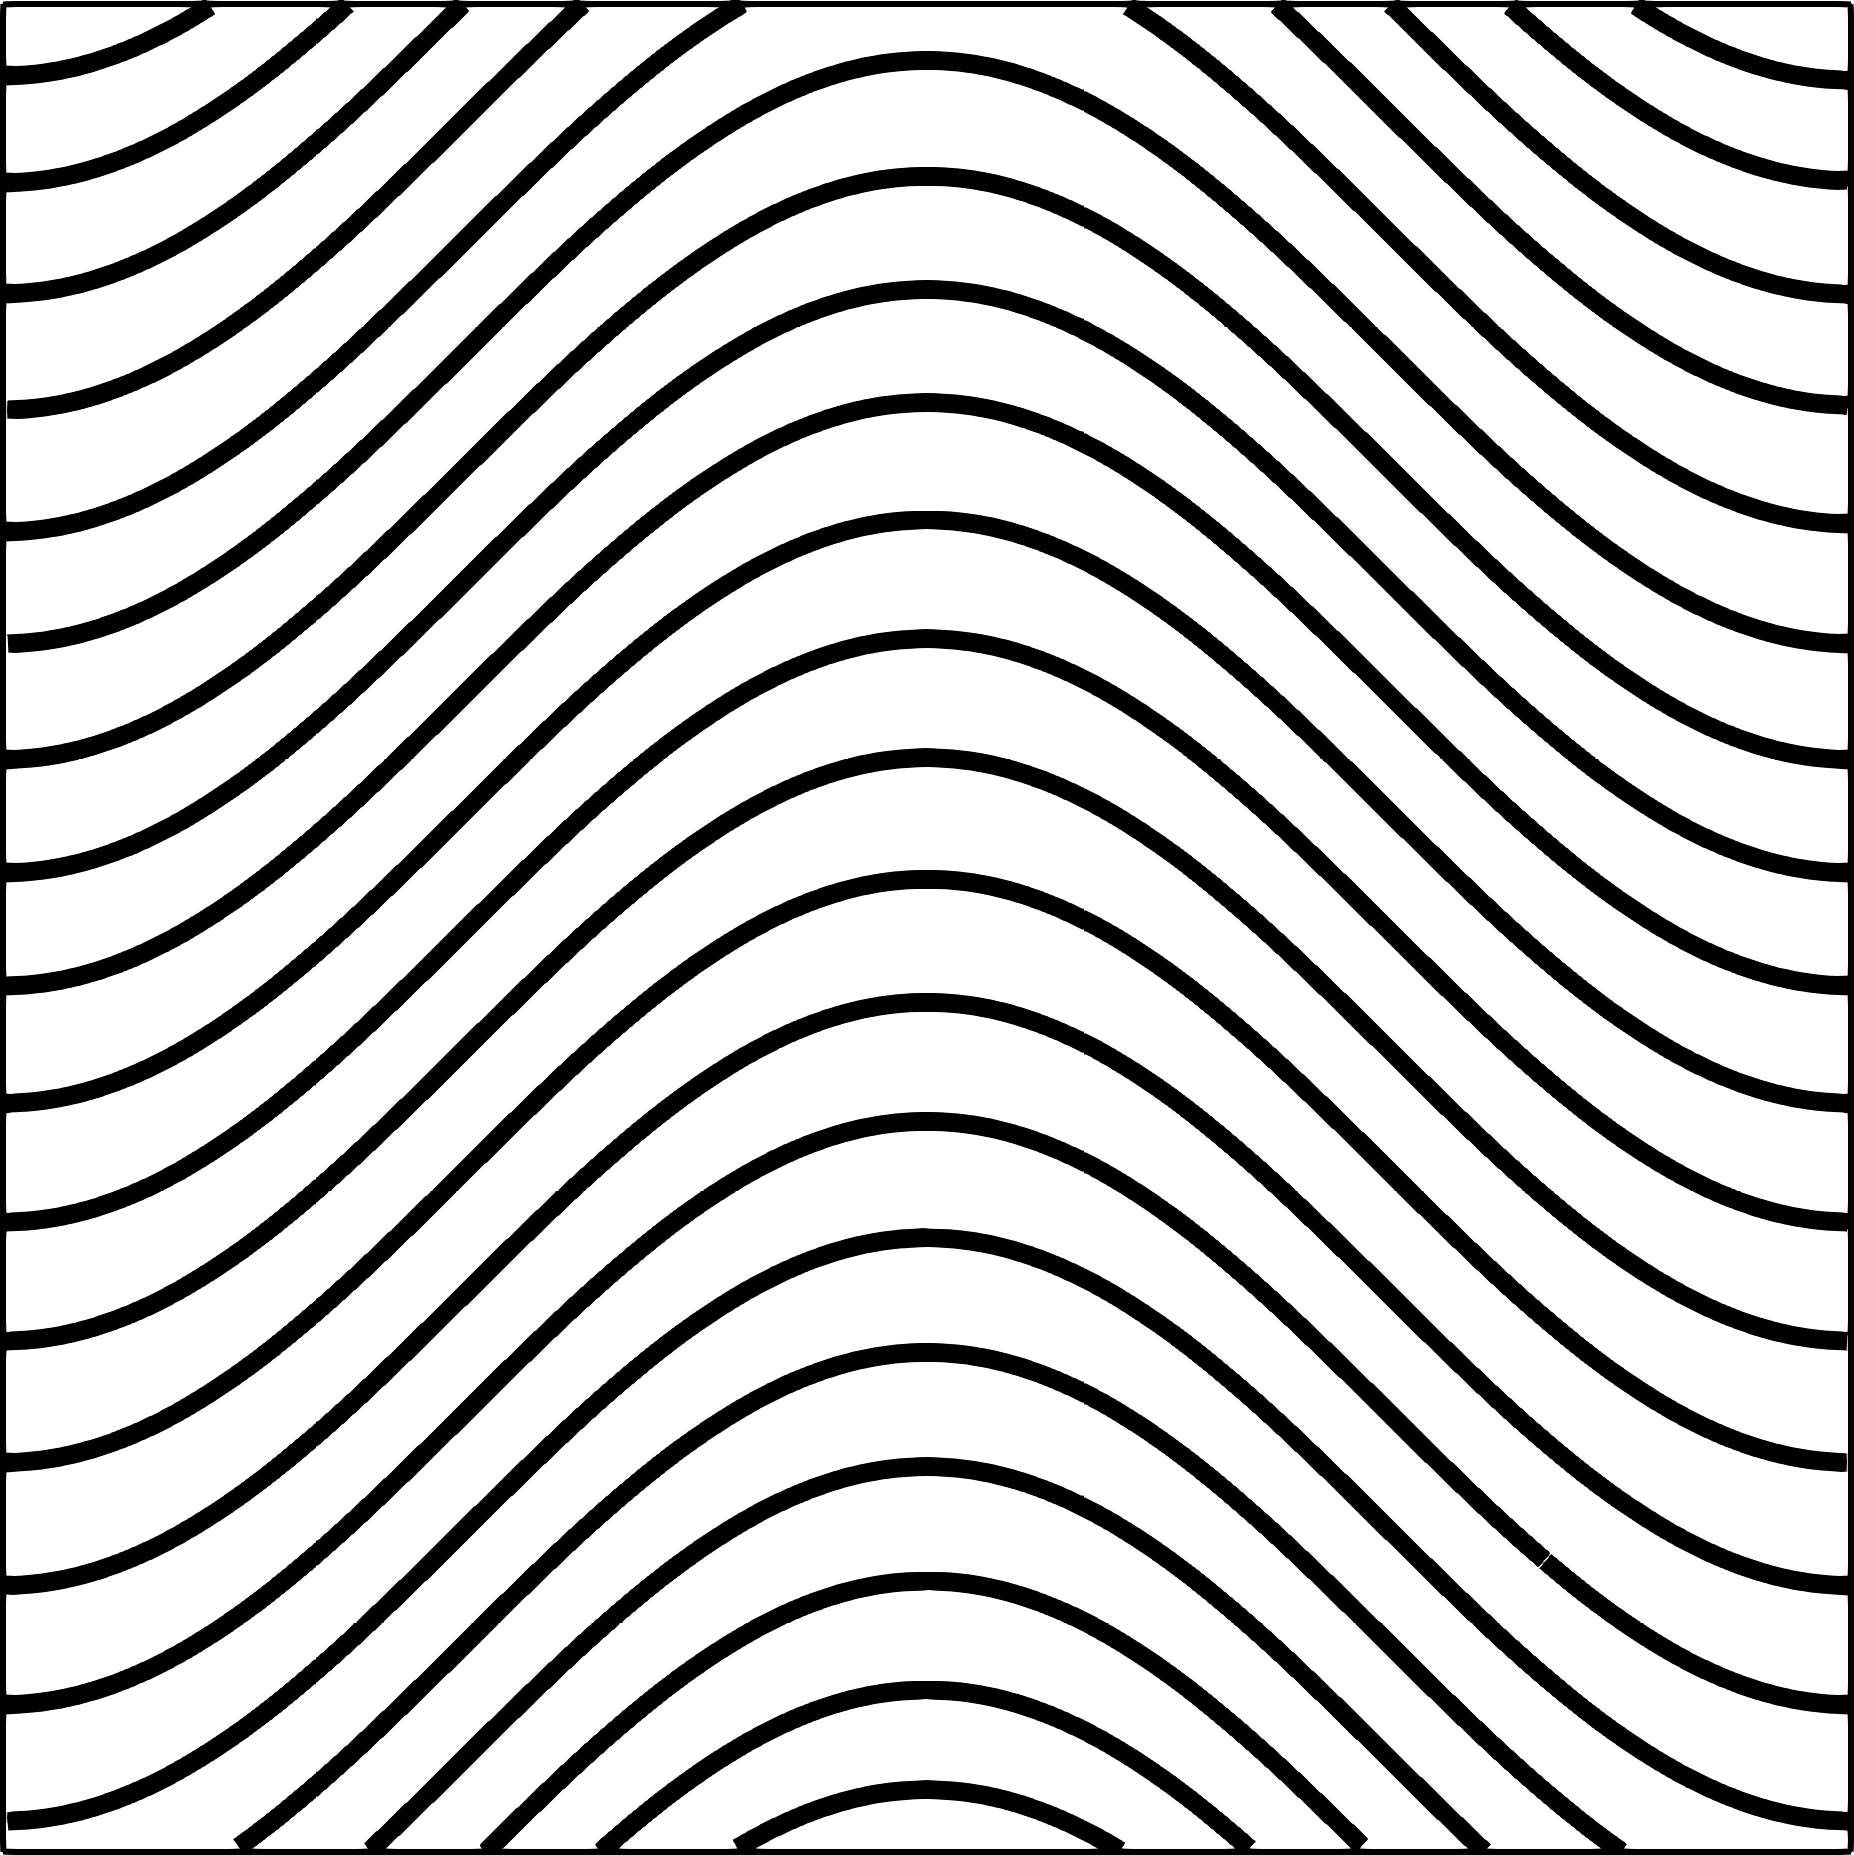
\includegraphics[scale=.08]{figures/WavesStreamlines.png}
    \caption{A set of streamlines generated for the field in \Cref{fig:fundamentals_1}(a).}
    \label[figure]{fig:fundamentals_2}
\end{figure}
\subsection{Streamlines}
Given a vector field $u$ and a point $P$, we can trace the movement of this point through $u$ by integrating over the field.
Intuitively, we can step through the field by choosing the next point $P_n = P_{n-1} + c \cdot u(P_{n-1})$, with $c$ being a step size scale.
If we do this an infinite number of times with $\pm c$ close to zero,
we end up with a set of points $S$ we have passed through, which defines the streamline.
$S$ has two notable properties:
\begin{itemize}
    \item Every point $P\in S$ inside this set has a velocity equal to $u(P)$.
    Hence, a streamline is tangent to the vector field at every point.
    \item No matter which point inside $S$ we use as $P_0$, we will always obtain the same set $S$ as its streamline.
    Therefore, any point inside $S$ is a potential \textit{seed} yielding the streamline $S$.
\end{itemize}
\subsection{Spatial Coherence}
If we want to visualize a vector field, we want its features to be easily identifiable.
At the same time, we do not want to introduce distractions or artifacts due to the visualization technique.
The deciding factors of uniformity in streamline visualization are streamline length and density.
Longer streamlines make for a smoother appearance, whereas many short lines tend to obfuscate and hinder the recognition of important features like the aforementioned critical points.
\Cref{fig:fundamentals_2} shows strong spatial coherence.

\begin{figure}[t]
    \centering
    \begin{subfigure}{.29\textwidth}
        \centering
        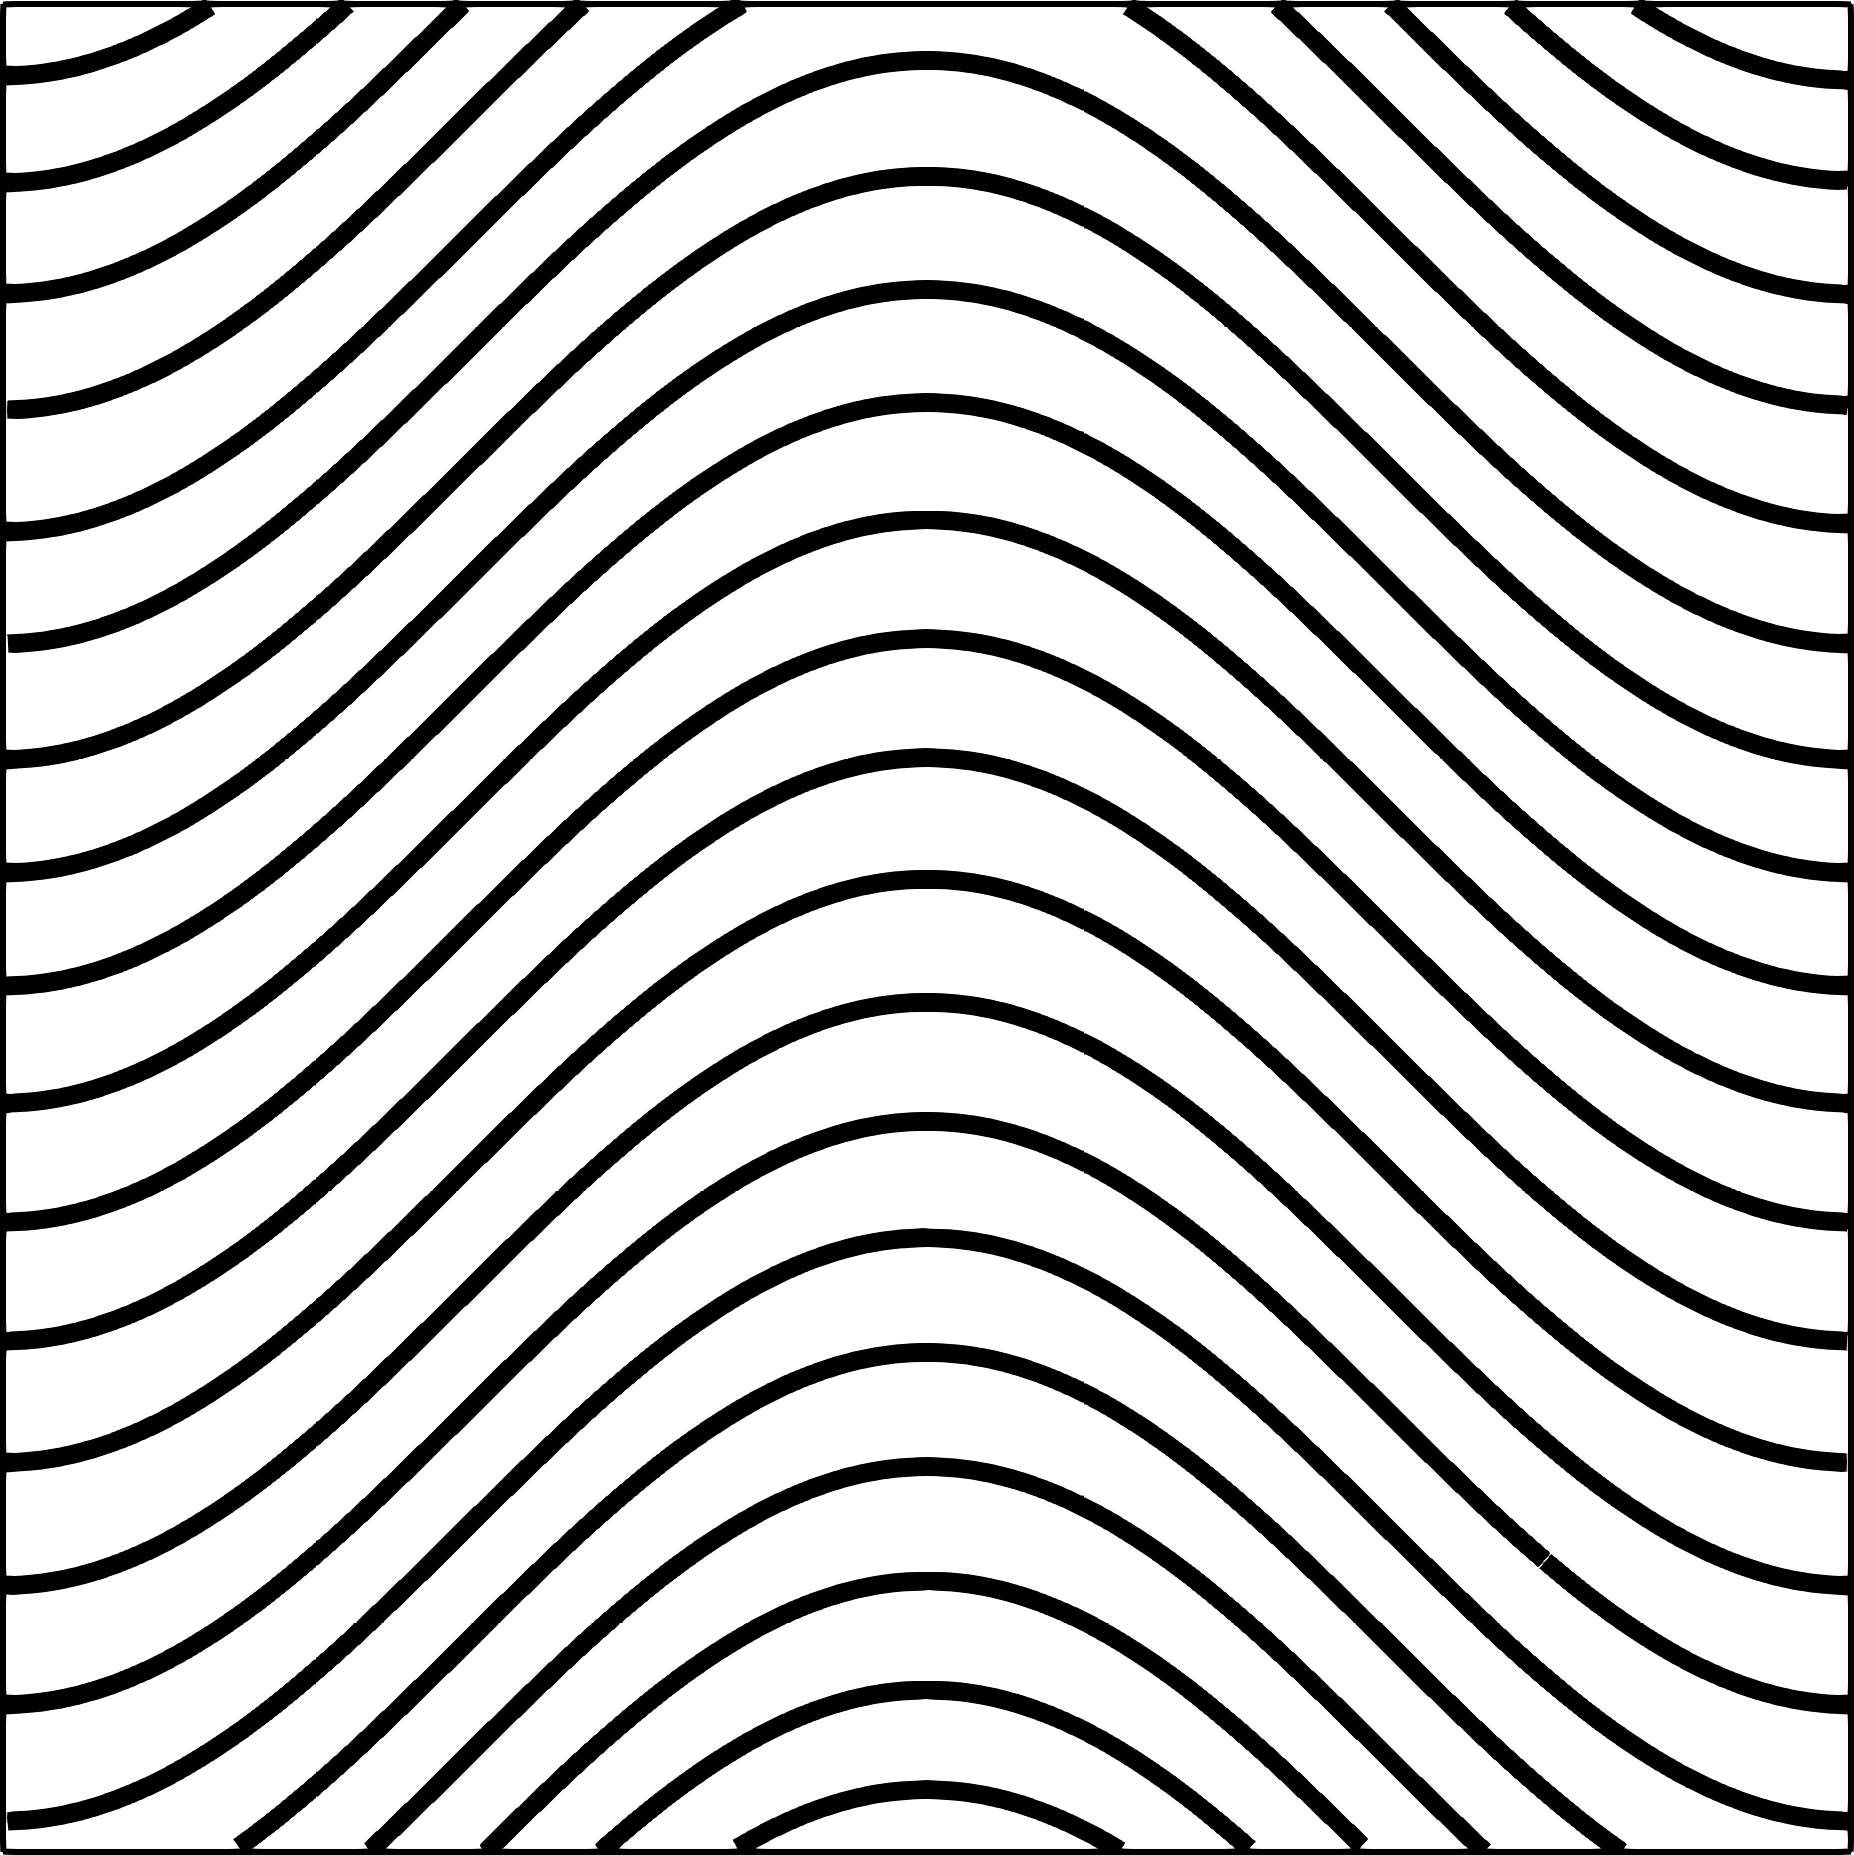
\includegraphics[scale=.08]{figures/WavesStreamlines.png}
        \caption{}
    \end{subfigure}
    \begin{subfigure}{.29\textwidth}
        \centering
        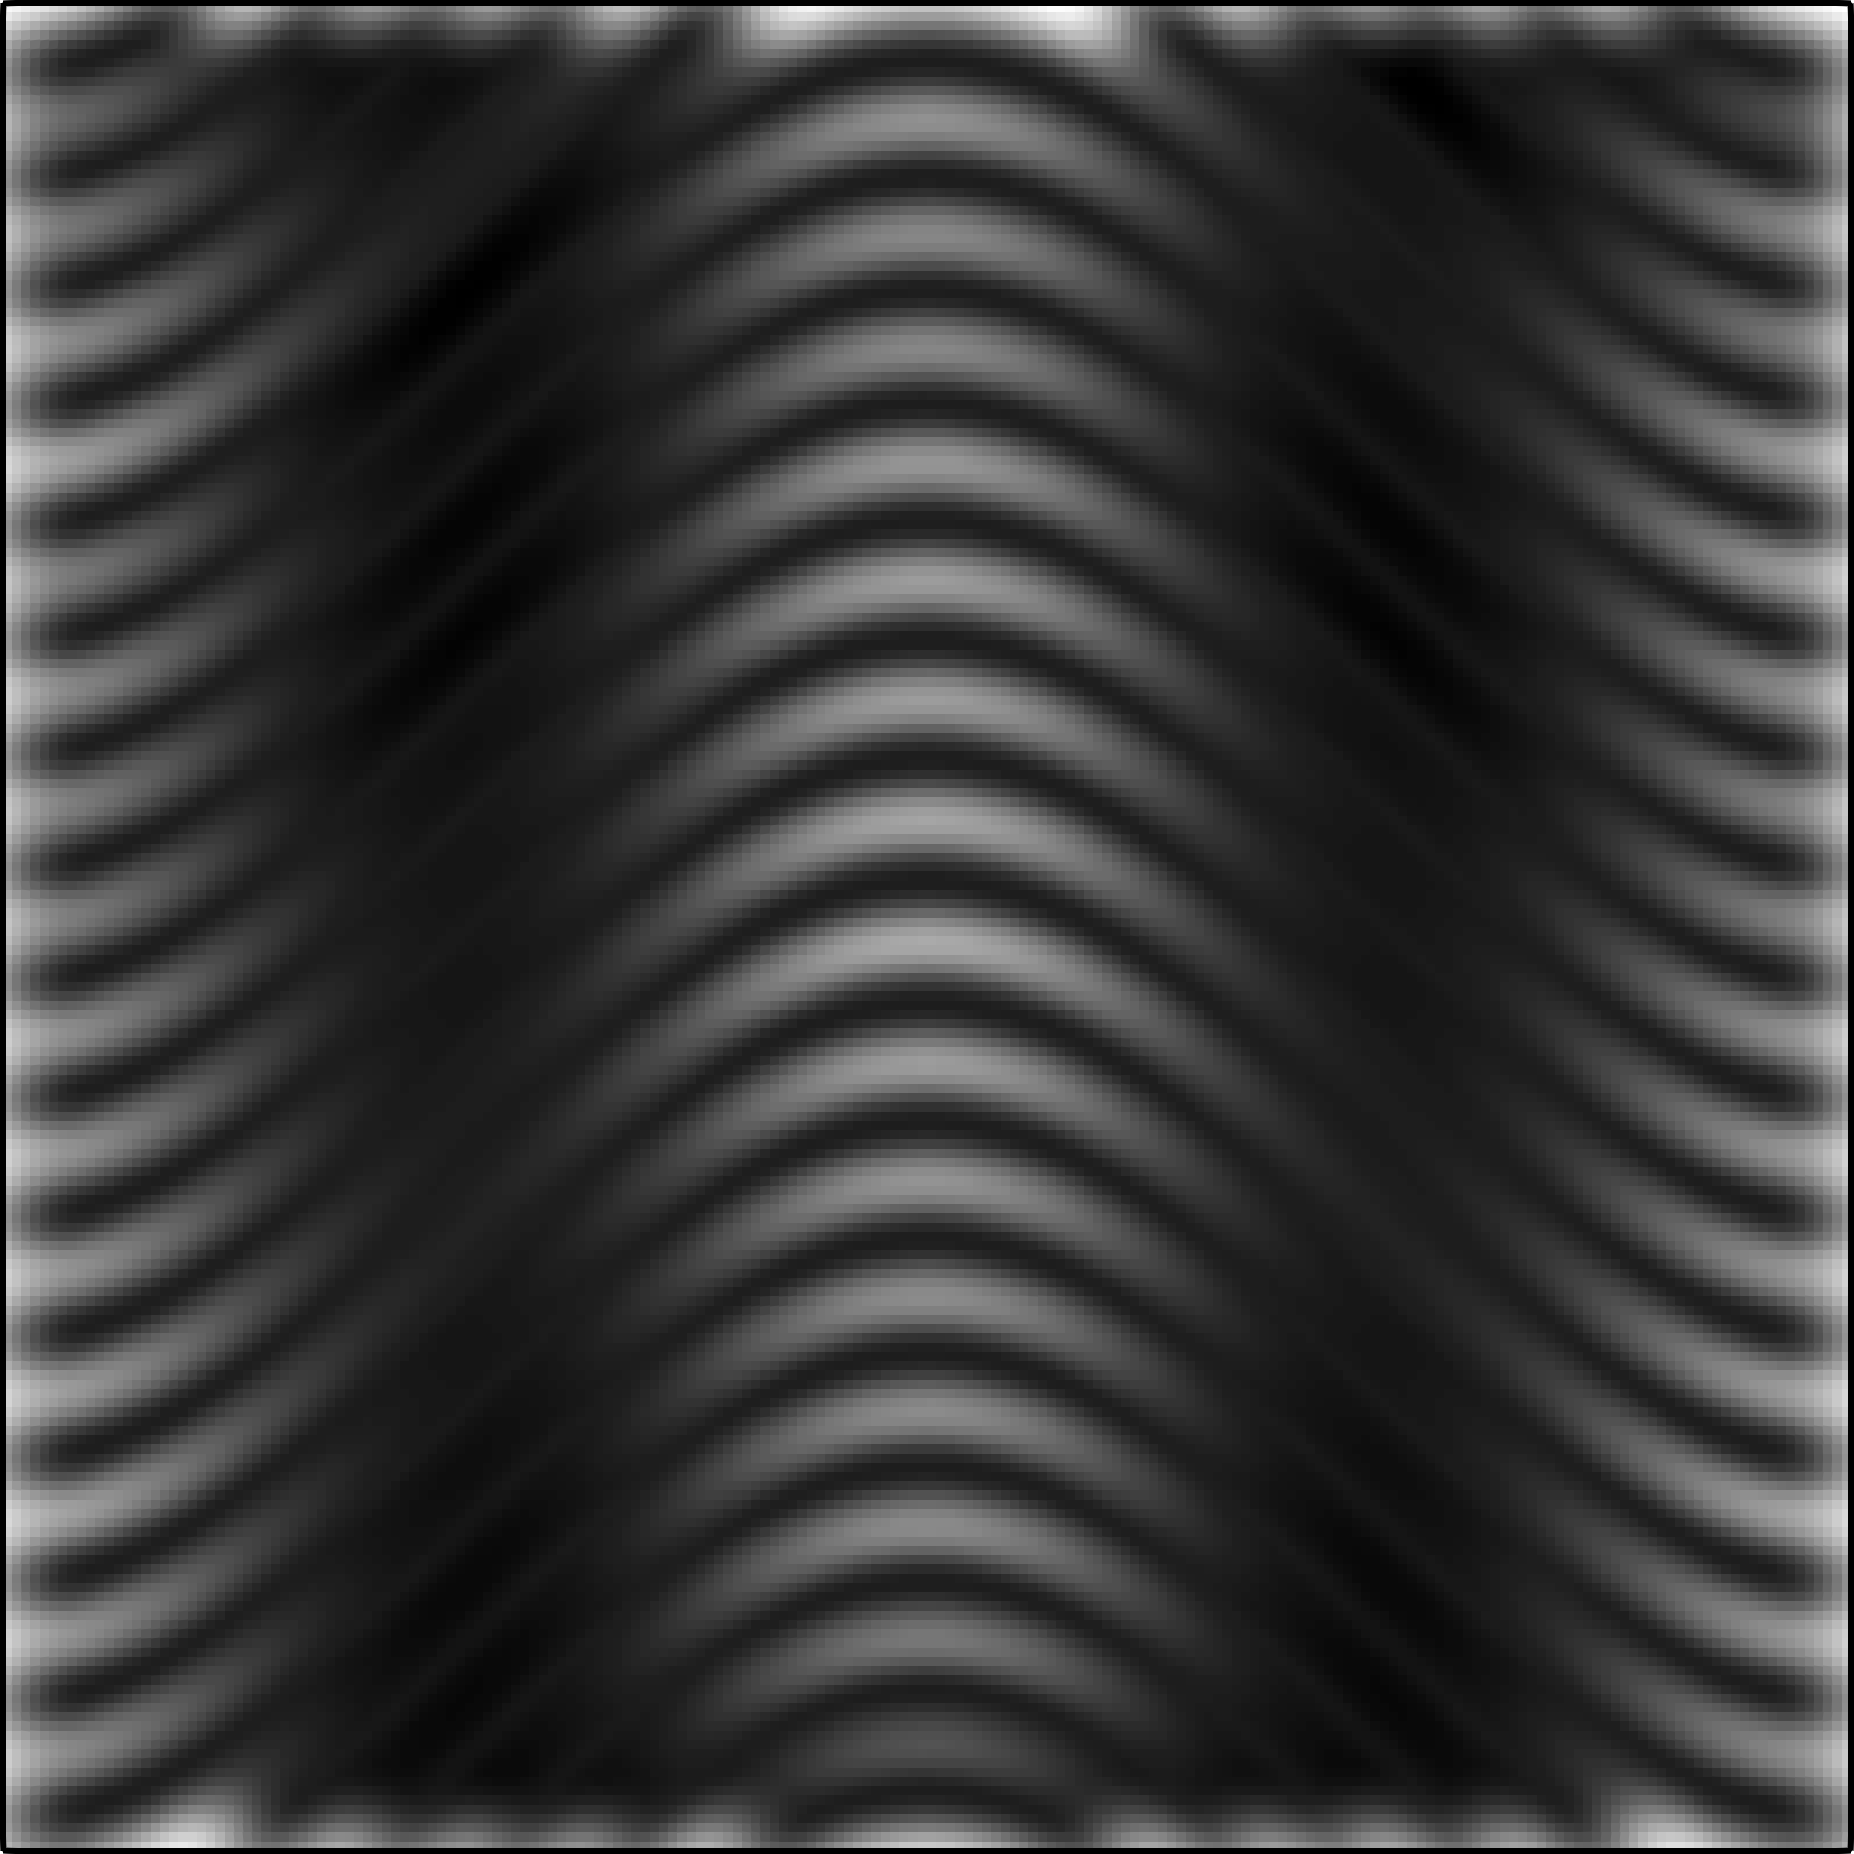
\includegraphics[scale=.08]{figures/WavesStreamlinesBlur.png}
        \caption{}
    \end{subfigure}
    \begin{subfigure}{.3\textwidth}
        \centering
        \setlength\pgfplotswidth{1.5\textwidth}
        \begin{tikzpicture}
    \def\r(#1){abs(#1) / 2}%
    \begin{axis}
        \addplot[color=blue, ultra thick, samples=100, domain=-2.5:2.5]{
            \r(x) < 1 ? 2*(\r(x))^3-3*(\r(x))^2+1 : 0
        };
        \addplot[color=red, dotted, ultra thick, domain=-2.5:2.5]{
            2*(\r(x))^3-3*(\r(x))^2+1
        };
    \end{axis}
\end{tikzpicture}
\begin{tikzpicture}[]
    \def\r(#1,#2){(((#1)^2 + (#2)^2) / 2)^0.5}%
    \def\K(#1,#2){2 * \r(#1,#2)^3 - 3 * \r(#1,#2)^2 + 1}
    \begin{axis}[
        % xmin=-2.5,xmax=2,
        % ymin=-2.5,ymax=2,
        zmin= 0  ,zmax=1,
        % axis line style={draw=none},
        % axis equal image,
    ]
    \addplot3[
        surf,
        domain=-2:2,
        samples=40
    ]
    % K(x,y) = 2r^3 - 3r^2 + 1 if r < 1 else 0
    % r = sqrt(x^2 + y^2) / R
    % R = desired radius, lets use 2
    % therefore we get:
    % r = sqrt(x^2 + y^2) / 2
    % K(x,y) = sqrt(x^2 + y^2) / 2 < 1 ? 2 * (sqrt(x^2 + y^2) / 2) ^ 3 - 3 * (sqrt(x^2 + y^2) / 2) ^ 2 + 1 : 0
    {\r(x,y) < 1 ? \K(x,y) : 0};% < 1 ? 2 * r(x,y) ^ 3 - 3 * r(x,y) ^ 2 + 1 : 0};
    \end{axis}
\end{tikzpicture}

        \caption{}
    \end{subfigure}
    \caption{
        A set of streamlines (a) generated for the field in \Cref{fig:fundamentals_1}(a).
        (b) Low-pass version of (a) after convolving it with a kernel like the one shown in (c).
    }
    \label[figure]{fig:fundamentals_3}
\end{figure}

\section{Image Processing}
In this thesis, we need to convolve an image with a cubic Hermitian kernel in order
to achieve a consistent blur with a specified falloff distance.
We therefore use some concepts from the field of image processing we briefly describe here.
\label[section]{sec:IP}
\subsection{Convolution} Convolution is a process often found in image- or signal processing.
For this thesis we focus on the former:
A kernel (\Cref{fig:fundamentals_3}(c)) is applied to every pixel in an image,
affecting it and other surrounding pixels by adding or subtracting its value at that position. 

\subsection{Blurring} Blurring  refers to a special type of convolution, making edges in an image less sharp.
Note the difference between black and white contrast for \Cref{fig:fundamentals_3}(a) and (b).

\begin{figure}[ht]
    \centering
    \begin{subfigure}[position]{.5\textwidth}
        \centering
        \setlength\pgfplotswidth{.9\textwidth}
        \begin{tikzpicture}
    \tikzset{
        pics/carc/.style args={#1:#2:#3}{
            code={
               \draw[pic actions] (#1:#3) arc(#1:#2:#3);
            }
        }
    }
    \begin{axis}[ 
        ticks=none,
        axis lines = middle,
        axis line style={->},
        ymin=-1.3, ymax=1.3,
        xmin=-1.3, xmax=1.3,
        xlabel={$1$},
        ylabel={$i$},
        width=\pgfplotswidth,
        height=\pgfplotswidth
        ]
        \draw (0,0) circle [radius=1, fill=white];
        \draw[very thick] (0,0) pic[red]{carc=0:72:2cm};
        \node[red] at (1,1) {$\frac{2\pi}{5}$};

        \draw[very thick, ->] (0,0) -- (1,0) node[midway, above right] {$n_0$};
        \draw[very thick, ->] (0,0) -- ( .309, .951) node[midway, right] {$n_1$};
        \draw[very thick, ->] (0,0) -- (-.809, .588) node[midway, above] {$n_2$};
        \draw[very thick, ->] (0,0) -- (-.809,-.588) node[midway, below] {$n_3$};
        \draw[very thick, ->] (0,0) -- ( .309,-.951) node[midway, right] {$n_4$};
    \end{axis}
\end{tikzpicture}

    \end{subfigure}
    \caption{The 5th roots of unity $n_0...n_4$ partition the unit circle equally}
    \label[figure]{fig:ROU}
\end{figure}

\section{Roots of Unity}
\label[section]{sec:ROU}
To extend our initial prototype from 2D to 3D, we need to be able to place uniformly spaced points
on a normal plane around a line segment.
To do this easily, we make use of the field of linear algebra and use the roots of unity.
\bigskip 

With $i$ being the complex number, we can use Euler's equation
\[n_j = e^{ji2\pi/k}, j = 0, 1, ..., k-1\] to obtain $k$ numbers
lying on the complex unit circle seen in \Cref{fig:ROU},
which are called the $k$-th roots of unity.
Notable properties are their length of exactly one, and that they divide the unit circle equally.
We can convert them to vectors in $\mathbb{R}^2$ using 
\[\vectr{v}_j = (\operatorname{Re}(n_j), \operatorname{Im}(n_j))^T\,.\]

% paar mehr beispiele, convolution etc, ausblick
% which algortimh?